%%%%%%%%%%%%%%%%%%%%%%%%%%%%%%%%%%%%%%%%%%%%%%%%%%%%%%%%%%%%%%%%%%%%%%%%%
% SJCIEE manuscript guide/template
% version 1.1, May 27, 2022. by T. Ueta
%%%%%%%%%%%%%%%%%%%%%%%%%%%%%%%%%%%%%%%%%%%%%%%%%%%%%%%%%%%%%%%%%%%%%%%%%
\documentclass[10pt,twocolumn]{jsarticle}            % for platex 
%\documentclass[10pt,twocolumn]{ltjsarticle}         % for lualatex 
\usepackage[top=30mm, bottom=25mm, left=18mm, right=18mm]{geometry}
\usepackage[bookmarks=false, colorlinks=true, 
	dvipdfmx,                        % comment this line out for lualatex 
	linkcolor=black, urlcolor=black, citecolor=black ]{hyperref}
\usepackage{newtxtext,newtxmath}
\usepackage{wrapfig}
\usepackage[dvipdfmx]{graphicx,xcolor}               % for platex
%\usepackage{graphicx,xcolor}                        % for lualatex 
\usepackage{secdot}
\usepackage{float}

\sectiondot{subsection}
\columnsep=12pt \columnseprule=0pt \jot=0pt
\topsep=0pt \parskip=0pt \parindent=12pt
\floatsep=10pt \textfloatsep=10pt \intextsep=10pt
\setlength{\abovedisplayskip}{10pt plus 5pt}
\setlength{\belowdisplayskip}{8pt plus 5pt}
\renewcommand{\textfraction}{0.1}
\renewcommand{\floatpagefraction}{0.1}
\renewcommand{\topfraction}{1.0}
\renewcommand{\baselinestretch}{0.9}
\makeatletter
\def\section{\@startsection {section}{1}{\z@}%
{1.0ex plus 0.5ex minus .2ex}{0.5ex plus .2ex}{\large\bfseries}}
\def\subsection{\@startsection{subsection}{2}{\z@}%
{0.7ex plus 0.3ex minus .2ex}{0.3ex plus .2ex}{\normalsize\bfseries}}
\def\subsubsection{\@startsection{subsubsection}{3}{\z@}%
{0.4ex plus 0.2ex minus .2ex}{0.2ex plus .2ex}{\normalsize}}
\renewenvironment{thebibliography}[1]{%
	\subsection*{\refname}\@mkboth{\refname}{\refname}%
	\list{\@biblabel{\@arabic\c@enumiv}}%
		{\settowidth\labelwidth{\@biblabel{#1}}%
		\leftmargin\labelwidth \advance\leftmargin\labelsep
		\setlength\baselineskip{13pt} \setlength\itemsep{0pt}
		\@openbib@code \usecounter{enumiv}%
		\let\p@enumiv\@empty \renewcommand\theenumiv{\@arabic\c@enumiv}}%
	\sloppy \clubpenalty4000 \@clubpenalty\clubpenalty
\widowpenalty4000 \sfcode`\.\@m}
{\def\@noitemerr {\@latex@warning{Empty `thebibliography' environment}}%
\endlist}
\makeatother
\pagestyle{empty}
%%%%%%%%%%%%%%%%%%%%%%%%%%%%%%%%%%%%%%%%%%%%%%%%%%%%%%%%%%%%%%%%%%%%%%%%%
% Please edit below
%%%%%%%%%%%%%%%%%%%%%%%%%%%%%%%%%%%%%%%%%%%%%%%%%%%%%%%%%%%%%%%%%%%%%%%%%
\begin{document}

\twocolumn[
\begin{center}
{\Large 
% 講演番号刷り入れ用余白を作るために\rule で空白を挿入しています.
% 刷り上がりを見ながら50mm * 45mm の空白を確保してください.
\rule{0mm}{0mm}ゲノム選抜のための双曲埋め込みの検討\\
Exploring Hyperbolic Embedding for Genomic Selection\\
}
\vspace*{3pt} 
{ \large
\begin{tabular}{ccccc}
森 樹伸${}^1$ & 木脇 太一${}^1$ & 小林 栄治${}^2$ & 大江 美香${}^2$ & 荒川 愛作${}^2$ \\ 
S. Mori${}^1$ & T. Kiwaki${}^1$ & E. Kobayashi${}^2$ & M. Ooe${}^2$ & A. Arakawa${}^2$ \\
\end{tabular}\\
\begin{tabular}{cccc}
近森 太志${}^3$ & 濱田 和希${}^3$ & 山口 亜利沙${}^1$ & 松川 和嗣${}^1$\\
T. Chikamori${}^3$ & K. Hamada${}^3$& A. Yamaguchi${}^1$& K. Matukawa${}^1$\\
\end{tabular}\\
(高知大学${}^1$, 農研機構${}^2$, 高知県畜産試験場${}^3$)
}
\end{center}
\vspace*{12pt} 
]

\section{背景}
近年,畜産分野では,ゲノム情報を用いた育種,すなわちゲノム選抜(GS)が盛んに行われている.
GSでは,形質とゲノムの間の非線形な関係を捉えるために,機械学習を応用する研究が注目されているが,
従来の線形モデルと比べ予測精度が常に優れているわけではない.

その一因として,ゲノムデータ特有の高次元・小サンプル問題が挙げられ,過学習などの問題を引き起こす.
このため,次元削減などの前処理が重要な役割を果たす.

そこで本研究では,ゲノムデータが持つ潜在的な階層構造に着目し,
階層構造の表現に優れる双曲空間への埋め込みを適用することで,
データを従来よりも低次元で表現し,
前述の問題の緩和を目指す.
なお,本稿では,埋め込み手法の一つ HypHC\cite{hypHC}の実装結果について報告する.

\section{双曲埋め込み}
\subsection{双曲空間}
双曲空間は,一定の負の曲率をもつ非ユークリッド空間であり,
半径の増加に伴い体積が指数的に増加する特性を持つ.
これにより,階層が深まるにつれてノード数が指数的に増加する木構造(階層構造の一種)を自然に表現できるため,
階層構造の表現に優れているとされる.

双曲空間を表現するモデルはいくつか存在する.
例えば,Poincaré ball モデルは $\mathbb{B}^n=\{x\in\mathbb{R}^n\mid\|x\|<1\}$ と定義され,
単位球内で双曲空間を表現する.

\subsection{HypHC}
HypHCは,双曲空間(Poincaré ball モデル)上で階層クラスタリング(HC)的にデータを表現するための埋め込み手法である.
HCは類似度に基づいて,集団の構造を二分木で可視化する手法で,
類似度の高いペアは木の深部で,類似度の低いペアは根近くで結合するという方針を持つ.

Dasguptaのコスト関数は,この方針が木全体でどの程度達成されているかを評価する指標であり,
HypHCは,埋め込みから再構築される二分木のコストを最小化するように埋め込みを最適化する.

\section{土佐あかうしのSNPデータ}
本研究では,土佐あかうしのゲノムデータ,特に,
SNP(一塩基多型)データを使用する.
欠損値処理を行った結果,サンプル数 669 頭,次元数 58,995 SNPとなった.
現時点で,他手法で必要となる関連データは入手できなかったため,
SNP のみで実装可能である HypHC を選択した.
なお,非類似度としてユークリッド距離を用いた.

\section{結果}
\begin{wrapfigure}[12]{l}{40mm}
\centering
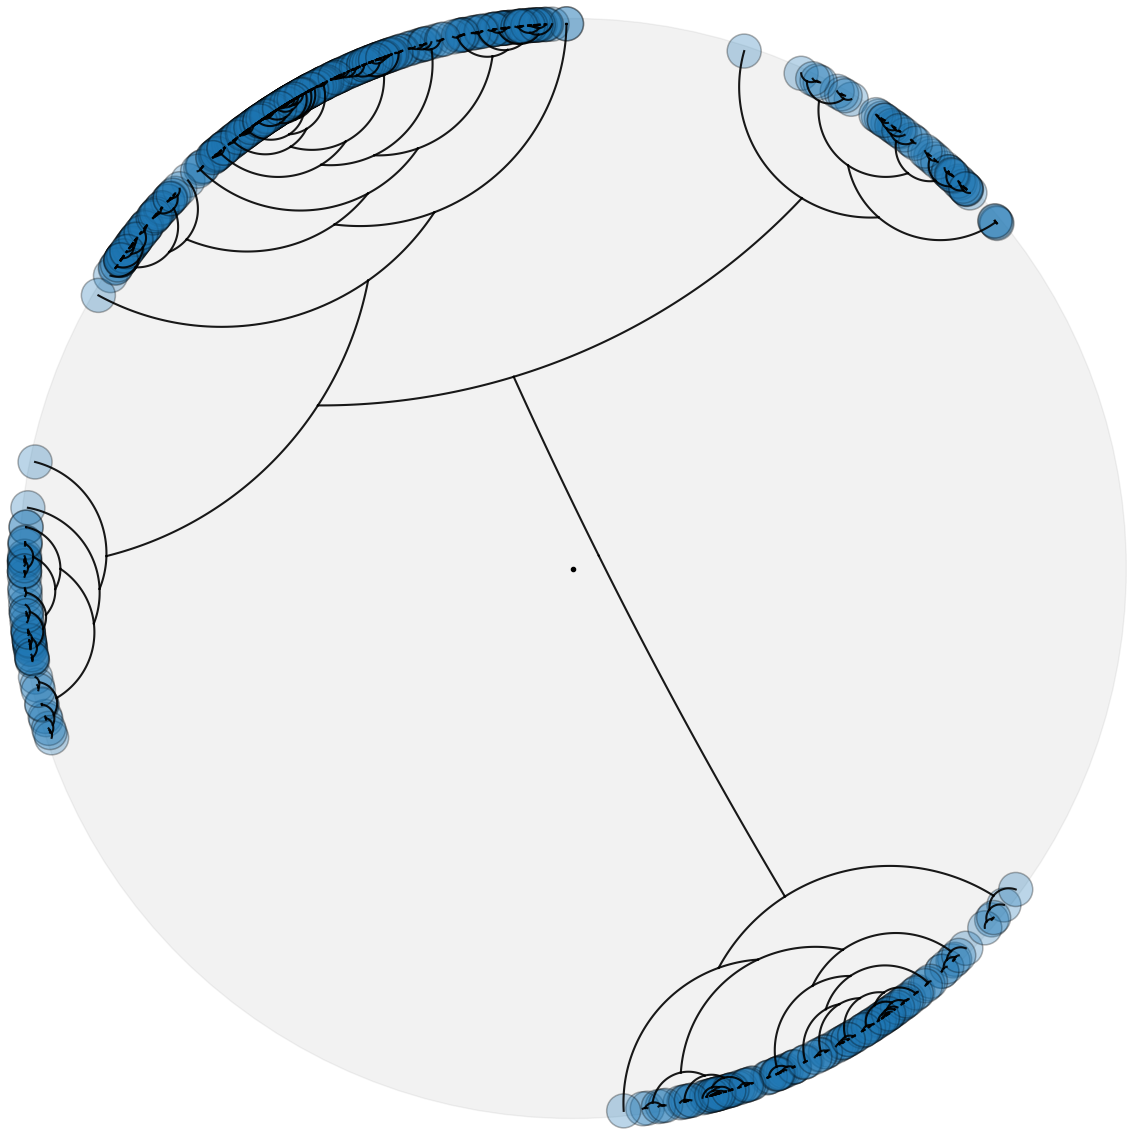
\includegraphics[width=43mm]{fig/SJCIEE_1.png}
\caption{HypHC (2 次元) の結果}
\label{fig:Embedding result}
\end{wrapfigure}
2 次元の双曲埋め込みの結果を図\ref{fig:Embedding result}に示す.
灰色の単位円がPoincaré ball モデルであり,青色の点が埋め込まれたデータ,実線が再構築された木を表す.
木には 4 つのクラスタが見られた.

表\ref{tab:d cost}に 再構築された木の Dasgupta のコストと,
HC の複数の構築方法(Ward,単,平均,完全)の中で最小のコストとなった ward法のコストを示す.
なお,埋め込み先の次元を増やすとコストはさらに改善したが,
50 次元以上では改善が見られなかった.


\begin{table}[H]
	\centering
	\caption{Dasguptaのコストの比較}
	\label{tab:d cost}
	\begin{tabular}{|c|c|}
			\hline
			 & Dasgupta's cost ($\times 10^{10}$)  \\
			\hline
			HypHC (2 次元) & $-5.87$ \\
			HypHC (50 次元) & $-5.91$  \\
			\hline
			HC (Ward 法) & $-5.75$  \\
			\hline
	\end{tabular}
\end{table}

\section{考察・展望}
図\ref{fig:Embedding result}で 4 クラスタが見られたが,
これが何を意味するかは,血統情報などとの関係を調べ明らかにする必要がある.
また,50 次元の埋め込みでコストの改善が収束したことから,
HypHC では,50次元への次元削減を達成したと考えられる.
いずれにせよ,埋め込みの良し悪しは,
GSにおける予測精度で評価するべきであり,今後の課題とする.

\begin{thebibliography}{9}
% \bibitem{review} 
% N. Chafai, I. Hayah, I. Houaga and B. Badaoui, 
% ``A review of machine learning  models applied to genomic  prediction in animal breeding,''
% \textsl{Frontiers in Genetics}, vol. 14, article 1150596, 2023.
%
\bibitem{hypHC} 
I. Chami, A. Gu, V. Chatziafratis and C. Ré, 
``From Trees to Continuous Embeddings and Back:  Hyperbolic Hierarchical Clustering,''
\textsl{NeurIPS}, vol. 33, pp. 15065 - 15076, 2020.
%
% \bibitem{web}
% 電気・電子・情報関係学会四国支部連合大会, 
% \url{https://sjciee.org} (2021年5月15日 参照)
\end{thebibliography}

\end{document}
